\documentclass[11pt, oneside]{amsart}   	% use "amsart" instead of "article" for AMSLaTeX format
\usepackage{geometry}                		% See geometry.pdf to learn the layout options. There are lots.
\geometry{letterpaper}                   		% ... or a4paper or a5paper or ... 
%\geometry{landscape}                		% Activate for for rotated page geometry
%\usepackage[parfill]{parskip}    		% Activate to begin paragraphs with an empty line rather than an indent
\usepackage{graphicx}				% Use pdf, png, jpg, or eps with pdflatex; use eps in DVI mode
								% TeX will automatically convert eps --> pdf in pdflatex		
\usepackage{amssymb}
\usepackage{amsmath}
\usepackage{subfig}
\usepackage{courier}
\newcommand{\us}{\textunderscore}


\title{COVID-19 Individual-Based Model with Instantaneous Contract Tracing}
\author{Rob Hinch, Will Probert, Anel Nurtay, Christophe Fraser}
%\date{}							% Activate to display a given date or no date

\begin{document}
\maketitle

\section{Overview}
COVID19-IBM is an individual-based model (IBM) for simulating an outbreak of COVID-19 in a city and to analyse the effect of both passive and active intervention strategies.
The model includes demographic data, which control both the dynamics of the interactions of individuals as well as disease outcomes.
Within the model, the virus (SARS-CoV-2) is spread via interactions between individuals.  Interactions can be remembered in the model to facilitate contact-tracing.
Intervention strategies such as self-quarantining, testing and contact-tracing can then be analysed.

\section{Demographics}

Demographics of the modelled population are based upon UK-wide data for 2018 from the Office of National Statistics (ONS). 
Three age categories are modelled: children (0-17 years), adults (18-64 years) and the elderly (65+).
Every individual is part of household which forms an important part of each person's daily interactions.
Data on household size is from the ONS.

\begin{table}[!htbp]
\centering
\begin{tabular}{ |p{3cm}|p{7cm}|p{1.2cm}|  }
 \hline
 \multicolumn{3}{|c|}{Demographic Parameters} \\
 \hline
 Name   & Description & Value \\
 \hline
 \hline 
 \texttt{n\us total}    & Total population simulated  & 100,000  \\
\hline
\texttt{uk\us pop\us 0\us 17}    & UK population 0-17 years old  (millions)  & 14.05 \\
\texttt{uk\us pop\us 18\us 64}  & UK population 18-64 years old  (millions)  & 40.22 \\
\texttt{uk\us pop\us 65}        & UK population 65+ years old (millions)       & 10.04 \\
 \hline 
\texttt{uk\us house\us1} & UK households with 1 person (thousands) & 8,198 \\
\texttt{uk\us house\us2} & UK households with 2 person (thousands) & 9,609 \\
\texttt{uk\us house\us3} & UK households with 3 person (thousands) & 4,287 \\
\texttt{uk\us house\us4} & UK households with 4 person (thousands) & 3,881 \\
\texttt{uk\us house\us5} & UK households with 5 person (thousands) & 1,254 \\
\texttt{uk\us house\us6} & UK households with 6 person (thousands) & 596 \\
 \hline
\end{tabular}
\end{table}
\medskip \medskip

\section{Interaction Network}

Interactions between individuals are modelled via membership of numerous networks which represent people's daily interactions.
An individual's membership to different networks leads to age-group assortativity in the interactions.
Previous studies of social contacts for infectious disease modelling have estimated the mean number of interactions that individual's have, stratified by age group (Mossong et al., 2008).
Mean interactions by age-group are estimated by aggregating this data.  We use the term "interactions" between individuals to mean possible contact that can spread disease.  We use the term "connections" between individuals as a superset of possible "interactions".  The modelled networks represent all the connections between individuals.  

\medskip \medskip
\begin{table}[!htbp]
\centering
\begin{tabular}{ |p{5cm}|p{1.5cm}|  }
 \hline
 \multicolumn{2}{|c|}{Mean daily interactions} \\
 \hline
Age group  & Value \\
 \hline
 \hline 
Children (0-17 years) & 15 \\
Adults (18-64 years) & 13 \\
Elderly (65 years+) & 7 \\
 \hline
\end{tabular}
\end{table}
\medskip \medskip

The model contains 3 types of networks: households, work-places (for children this would represent school) and random daily interactions.  Each simulated individual is a member of one of each type of network.  

\subsection{Household Network}
Each individual is assigned to live in a single household.  The proportion of people in each household is informed using UK household data (see Demographics section).
Each day every person has an interaction with everybody within their household.
Elderly people are assumed to live in either a 1 or 2 person household with other elderly people, with the ratio of elderly 1 and 2 person households being the same as the general population.
Children are assumed to live in household with two adults (so they can only live in 3/4/5/6 person households). 
The proportion of 3/4/5/6 person-households with children is the same as the those with adults only.

\subsection{Work-place Network}
Each individual is part of a single work-place network.
Work-place networks are modelled as Watts-Strogatz small-world networks (Watts and Strogatz, 1998).
A work-place network is modelled for each age group, with the network for children and elderly  containing a small proportion of adults (i.e.\ teachers and carers).
When constructing work-place networks individuals are randomly sorted, to ensure there is no unanticipated relationship between the household interactions and the local interactions on the small-world network.
Each day every person interacts with a random subset of their connections on their work-place network.

\medskip \medskip
\begin{table}[!htbp]
\centering
\begin{tabular}{ |p{6.3cm}|p{6.8cm}|p{1cm}|  }
 \hline
 \multicolumn{3}{|c|}{Work-place Network Parameters} \\
 \hline
 Name   & Description & Value \\
 \hline
 \hline 
\texttt{mean\us work\us interaction\us child}    & Mean number of connections for children & 10 \\
\texttt{mean\us work\us interaction\us adult}  & Mean number of connections for adults & 7 \\
\texttt{mean\us work\us interaction\us elderly} & Mean number of connections for elderly & 3 \\
\hline
\texttt{child\us network\us adults} & Fraction of adults in child network & 0.2 \\
\texttt{elderly\us network\us adults} & Fraction of adults in elderly network & 0.2 \\
\hline
\texttt{daily\us fraction\us work} & Fraction of daily work connections made & 0.5 \\
\texttt{prob\us network\us rewire}$^*$ & Probability of rewiring a connection in the Watts-Stogatz small-world network & 0.1 \\ 
 \hline
\end{tabular}
\end{table}
\medskip \medskip

The difference in the number of interactions for each age group is due to the overall number of daily interactions that each group have.  

\subsection{Random Network}

In addition to the structured networks of households and work-places, within which recurring daily interactions may occur, a number of random interactions are also included.  
Random interactions are drawn each day and are independent of the previous day's connections.
The number of random connections an individual makes is the same each day (without interventions) and is drawn at the start of the simulation from a negative-binomial distribution.
This variation in the number of interactions introduces "super-spreaders" into the network who have a much larger numbers of interactions than the average individual.

\medskip \medskip
\begin{table}[!htbp]
\centering
\begin{tabular}{ |p{7.2cm}|p{6.8cm}|p{0.9cm}|  }
 \hline
 \multicolumn{3}{|c|}{Random Network Parameters} \\
 \hline
 Name   & Description & Value \\
 \hline
 \hline 
\texttt{mean\us random\us interaction\us child}    & Mean number of connections for children & 2 \\
\texttt{mean\us random\us interaction\us adult}    & Mean number of connections for adults & 4 \\
\texttt{mean\us random\us interaction\us elderly} & Mean number of connections for elderly & 3 \\
\hline
\texttt{sd\us random\us interaction\us child}$^*$  & s.d.\ number of connections for children & 2 \\
\texttt{sd\us random\us interaction\us adult}$^*$ & s.d.\ number of connections for adults & 4 \\
\texttt{sd\us random\us interaction\us elderly}$^*$ & s.d.\ number of connections for elderly & 3 \\
 \hline
\end{tabular}
\end{table}
\medskip \medskip

The mean numbers of random connections were chosen so that the total number of daily interactions matched that from the social interaction studies. 
The split between work and random interactions was chosen to be lower in children. 
Each day a list is made which contains all individuals who make random interactions and each person is repeated by the number of interactions they make.
This list is then randomly shuffled and interactions are made between adjacent pairs on the shuffled list.

\section{Infection Dynamics}

COVID-19 is spread by interactions between infected and susceptible individuals.
The probability of transmission is determined by the infection status of the infected individual and the age of the susceptible.
Note that the type of interactions (i.e.\ household, work or random) or the length of the interaction (currently not modelled) is not used in deciding the likelihood of transmission.
Following evidence from early studies of the COVID19 outbreak and analyses of other epidemics of similar pathogens, it is assumed that immediately after become infected an individual is not infectious.
The level of infectiousness increases with time and peaks typically 5-7 days after the initial infection before decreasing.  
Following Fraser et al., (2004), we model infectiousness since time of infection using a gamma function, and the infectiousness on day $t$ after infection is calculated by integrating the gamma function from $t-1$ to $t$.
It has been observed that some people who are infected with SARS-CoV-2 remain asymptomatic and it is assumed that these people are less infectious than those who eventually develop symptoms.
Note that the model distinguishes between asymptomatic individuals who never develop symptoms, and individuals who are pre-symptomatic but who eventually develop symptoms.

Heterogeneity in susceptibility also plays a factor in transmission.  Data from the Chinese CDC suggest that the children are far less susceptible to infection than adults, and that the elderly are more susceptible than adults.  The model accounts for differences in susceptibility by a simple multiplicative factor based upon the age group of the susceptible individual.

The final formula for the probability of the virus being transmitted in a single interaction is
\begin{equation}
\lambda(t,a_s,b) = \frac{R s_{a_s}A_b}{ \bar I_{a_s}} \int_{t-1}^t f_{\Gamma}(u; \mu_i,\sigma_i^2) {\rm d}u,
\end{equation}
where $f_{\Gamma}(u; \mu_i,\sigma_i^2)$ is the p.d.f.\ of a gamma distribution with mean $\mu$ and variance $\sigma^2$; $t$ is the number of days since the infector become infected; $a_s$ is the age group of the susceptible; $b$ is an indicator of whether the infected individual is asymptomatic; the other terms listed in the Infectious Parameters table.  

The epidemic is seeded by randomly infecting a small number of individuals at the start of the infection.  Seed cases are assumed to have been infected immediately before the simulation starts.

\medskip \medskip
\begin{table}
\centering
\begin{tabular}{ |p{1.2cm}|p{6.8cm}|p{6.5cm}|p{1.2cm}|  }
 \hline
 \multicolumn{4}{|c|}{Infection Parameters} \\
 \hline
 Symbol & Name   & Description & Value \\
 \hline
 \hline 
$R$ & \texttt{infectious\us rate} & mean number of people infected by each infected person & 2.5 \\
$A_{\rm sym}$ &  - & relative infectious rate of symptomatic & 1 \\
$A_{\rm asym}$ & \texttt{asymptomatic\us infectious\us factor}& relative infectious rate of asymptomatic & 0.25 \\
 \hline
 $\mu_i$ &  \texttt{mean\us infectious\us period} & time of peak infectiousness (i.e.\ the mean of the gamma p.d.f.) & 6 days\\
 $\sigma_i$ &  \texttt{sd\us infectious\us period} & width of infectiousness curve (i.e.\ the s.d.\ of the gamma p.d.f.) & 2 days\\
 \hline
 $s_{\rm child}$   &  \texttt{relative\us susceptibility\us child} & relative susceptibility of child to adult & 0.1 \\
 $s_{\rm adult}$   &   - &  - & 1\\
 $s_{\rm elderly}$ &  \texttt{relative\us susceptibility\us elderly} & relative susceptibility of elderly to adult & 1.7 \\
 \hline
  -&  \texttt{n\us seed\us infection} & number of individual randomly infected at start of simulation & 10 \\
 \hline

\end{tabular}
\end{table}
\medskip \medskip

\section{Disease Dynamics}

Upon infection, an individual enters a disease progression cascade where the outcome and rates of progression are dependent upon age of the infected person (figure \ref{diseaseDynamics}).
The first split is that only a fraction of individual who will develop symptoms, where a fraction ($\phi_{\rm asym}$) remain asymptomatic.
Those who are asymptomatic are infectious (at a lower level, see Infection Dynamics section) and will move to a recovered state after a time ($\tau_{\rm a,rec}$) drawn from a gamma distribution.
Once an individual is recovered we assume that they have lifelong immunity and cannot be reinfected.

For individual who will develop symptoms, they start by being in the pre-symptomatic state, where, whilst they will be able to transmit the disease to others, they will not be showing any symptoms. 
This is important for modelling interventions because individuals in this state would not be able self-isolate unless they had been contact-traced (or there was a complete shutdown).
After a time ($\tau_{\rm sym}$) drawn from a gamma distribution, the individual develops symptoms, at which case interventions can be triggered such as self-isolation, testing and contact-tracing.
Whilst most individuals will only develop mild symptoms, a fraction ($\phi_{\rm hosp}({\rm age})$) will go on to require hospitalisation, where the probability of requiring hospital treatment is age-dependent.
Those individuals who do not require hospitalisation will recover after a time ($\tau_{\rm rec}$) drawn from a gamma distribution, whilst those who require hospital treatment enter after a time ($\tau_{\rm hosp}$) drawn from a Bernoulli distribution of either 1 or 2 days.
Once entering hospital, a number of interventions can take place. 
We assume that a clinical diagnosis can immediately decide whether the patient is a case so that contract-tracing can be commenced straight away.
Of those who enter a hospital, a fraction ($\phi_{\rm death}({\rm age})$) will die with the rest recovering. 
The time to death ($\tau_{\rm death}$) and recovery ($\tau_{\rm death}$) are both drawn from gamma distributions.

The disease state transitions are shown in (figure \ref{diseaseDynamics}) and the model parameters are in the table Disease Dynamics Parameters.

\begin{figure}
\centering
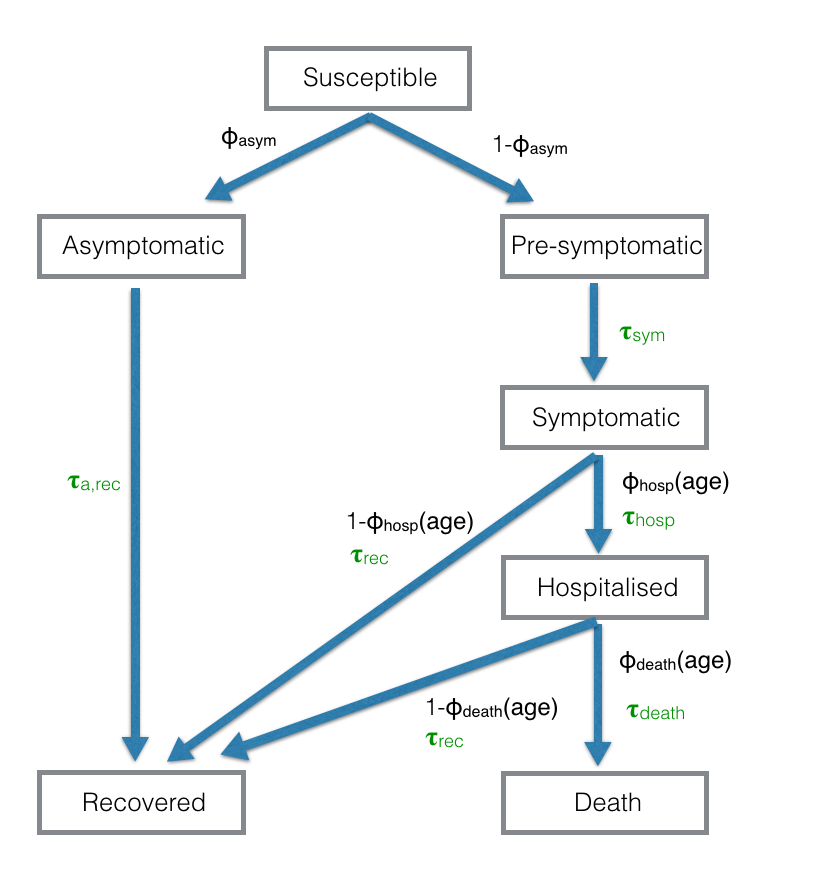
\includegraphics[width=.9\textwidth]{diseaseDynamics.png}
\caption{The disease status of an individual and the probability and time distribution of transitions. The $\phi_{\rm xxx}(\rm age)$ variables are the probability of transition to a particular state when there is a choice, where the probability depends upon the age of the individual.  The $\tau_{\rm xxx}$ are the gamma distributed variables of the time taken to make the transition.}
\label{diseaseDynamics}
\end{figure}

\medskip \medskip
\begin{table}
\centering
\begin{tabular}{ |p{2.3cm}|p{6.4cm}|p{4cm}|p{1.4cm}|  }
 \hline
 \multicolumn{4}{|c|}{Disease Dynamics Parameters} \\
 \hline
 Symbol & Name  & Description & Value \\
 \hline
 \hline 
  $\phi _{\rm asym} $  &  \texttt{fraction\us asymptomatic} & fraction of infected who are asymptomatic & 0.2 \\
 \hline
 $\phi_{\rm hosp} ({\rm child } )$     &  \texttt{hospitalised\us fraction\us child}    & fraction of symptomatic children hospitalised & 0.15 \\
 $\phi_{\rm hosp} ({\rm adult } )$    &  \texttt{hospitalised\us fraction\us adult}    & fraction of symptomatic adults hospitalised & 0.15 \\
 $\phi_{\rm hosp} ({\rm elderly } )$ &  \texttt{hospitalised\us fraction\us elderly} & fraction of symptomatic elderly hospitalised & 0.25 \\
 \hline
 $\phi_{\rm death} ({\rm child } )$    &  \texttt{fatality\us fraction\us child}     & fraction of hospitalised children who die & 0.01 \\
 $\phi_{\rm death} ({\rm adult } )$    &  \texttt{fatality\us fraction\us adult}    & fraction of hospitalised adults who die & 0.04 \\
 $\phi_{\rm death} ({\rm elderly } )$ &  \texttt{fatality\us fraction\us elderly} & fraction of hospitalised elderly who die & 0.25 \\
 \hline
$\mu_{\rm sym} $       &  \texttt{mean\us time\us to\us symptoms} & mean time to symptoms & 5.5 days \\
$\sigma_{\rm sym} $  &  \texttt{sd\us time\us to\us symptoms}       & s.d.\ time to symptoms & 2.5 days \\
 \hline
$\mu_{\rm sym} $       &  \texttt{mean\us time\us to\us symptoms} & mean time to symptoms & 5.5 days \\
$\sigma_{\rm sym} $  &  \texttt{sd\us time\us to\us symptoms}       & s.d.\ time to symptoms & 2.5 days \\
 \hline
$\mu_{\rm hosp} $       &  \texttt{mean\us time\us to\us hospital}  & mean time to hospital after showing symptoms & 1.6 days \\
 \hline
$\mu_{\rm death} $       &  \texttt{mean\us time\us to\us death} & mean time to death once hospitalised & 12 days \\
$\sigma_{\rm death} $  &  \texttt{sd\us time\us to\us death}       & s.d.\ time to death once hospitalised & 5 days \\
 \hline
$\mu_{\rm rec} $       &  \texttt{mean\us time\us to\us recover} & mean time to recover after symptoms/hospital &  12 days \\
$\sigma_{\rm rec} $  &  \texttt{sd\us time\us to\us recover}       & s.d.\ time to recover after symptoms/hospital & 5 days \\
 \hline
$\mu_{\rm a,rec} $       &  \texttt{mean\us asymptomatic\us to\us recover} & mean time to recover after asymptomatic &  15 days \\
$\sigma_{\rm a,rec} $  &  \texttt{sd\us asymptomatic\us to\us recover}       & s.d.\ time to recover after asymptomatic & 5 days \\
 \hline
\end{tabular}
\end{table}
\medskip \medskip

\section{Passive Interventions}

The model has the ability to model both passive and active interventions. 
Here we define an active intervention to be one involving contact-tracing with all other interventions being classed as passive.
Interventions are designed to reduce the rate of transmission, however, have the side-effect of potentially quarantining significant numbers of people. 
We also model the testing process to estimate the number of tests required by different intervention strategies.

\subsection{Hospitalisation} Upon hospitalisation, a patient immediately stops interacting with both their household and work-place networks. We also reduce the number of random interactions that they have. One aspect of the disease transmission that we are missing is that within hospitals and interactions with healthcare professionals. 

\subsection{Self-Isolation upon Symptoms}. The next type of intervention we model is self-isolation upon flu-like symptoms. In addition to those infected by coronavirus, we infect a random a sample of the population each day with non-coronavirus flu-like symptoms. Upon experiencing symptoms, a put a fraction of patients in to self-quarantine immediately. Quarantine is modelled by not interacting with your work-place network and having a much reduced number of connections on your random network. On entering self-quarantine, a coronavirus test is ordered for the following day and a result is delivered the day after. Given the patient is already presenting symptoms, we assume that the test will be 100\%. If the result tests positive then the individual remains in quarantine for 14 days (unless they require hospitalisation), otherwise they are released immediately.

\medskip \medskip
\begin{table}
\centering
\begin{tabular}{ |p{7.2cm}|p{6.8cm}|p{0.9cm}|  }
 \hline
 \multicolumn{3}{|c|}{Passive Intervention Parameters} \\
 \hline
 Name   & Description & Value \\
 \hline
 \hline 
\texttt{mean\us random\us interaction\us child}    & mean number of connections for children & 2 \\
\texttt{mean\us random\us interaction\us adult}    & mean number of connections for adults & 4 \\
\texttt{mean\us random\us interaction\us elderly} & mean number of connections for elderly & 3 \\
\hline
\texttt{sd\us random\us interaction\us child}$^*$  & s.d.\ number of connections for children & 2 \\
\texttt{sd\us random\us interaction\us adult}$^*$ & s.d.\ number of connections for adults & 4 \\
\texttt{sd\us random\us interaction\us elderly}$^*$ & s.d.\ number of connections for elderly & 3 \\
 \hline
\end{tabular}
\end{table}
\medskip \medskip


\section{Active Interventions}

\section{Implementation Details}

\section{References}


\end{document}  
